\documentclass{beamer}

% There are many different themes available for Beamer. A comprehensive
% list with examples is given here:
% http://deic.uab.es/~iblanes/beamer_gallery/index_by_theme.html
% You can uncomment the themes below if you would like to use a different
% one:
%\usetheme{AnnArbor}
%\usetheme{Antibes}
%\usetheme{Bergen}
%\usetheme{Berkeley}
%\usetheme{Berlin}
%\usetheme{Boadilla}
%\usetheme{boxes}
%\usetheme{CambridgeUS}
\usetheme{Copenhagen}
%\usetheme{Darmstadt}
%\usetheme{default}
%\usetheme{Frankfurt}
%\usetheme{Goettingen}
%\usetheme{Hannover}
%\usetheme{Ilmenau}
%\usetheme{JuanLesPins}
%\usetheme{Luebeck}
%\usetheme{Madrid}
%\usetheme{Malmoe}
%\usetheme{Marburg}
%\usetheme{Montpellier}
%\usetheme{PaloAlto}
%\usetheme{Pittsburgh}
%\usetheme{Rochester}
%\usetheme{Singapore}
%\usetheme{Szeged}
%\usetheme{Warsaw}
\usepackage{todonotes}
\usepackage{xcolor,colortbl}

\usepackage{tikz}
\usepackage{pgfplots}

\title{Multivariate Statistics and and Pattern Recognition}

% A subtitle is optional and this may be deleted
\subtitle{Exam Presentation - Skin Segmentation}

\author{Frederik~S.~Vanggaard~B\ae rentsen}
% - Give the names in the same order as the appear in the paper.
% - Use the \inst{?} command only if the authors have different
%   affiliation.

\institute[Aalborg University - Copenhagen] % (optional, but mostly needed)
{
  School of Information, Communication and Technology\\
  Aalborg University - Copenhagen}
% - Use the \inst command only if there are several affiliations.
% - Keep it simple, no one is interested in your street address.

\date{Fall 2014}
% - Either use conference name or its abbreviation.
% - Not really informative to the audience, more for people (including
%   yourself) who are reading the slides online

\subject{Multivariate Statistics and and Pattern Recognition}
% This is only inserted into the PDF information catalog. Can be left
% out. 

% If you have a file called "university-logo-filename.xxx", where xxx
% is a graphic format that can be processed by latex or pdflatex,
% resp., then you can add a logo as follows:

% \pgfdeclareimage[height=0.5cm]{university-logo}{university-logo-filename}
% \logo{\pgfuseimage{university-logo}}

% Delete this, if you do not want the table of contents to pop up at
% the beginning of each subsection:
\AtBeginSubsection[]
{
  \begin{frame}<beamer>{Outline}
    \tableofcontents[currentsection,currentsubsection]
  \end{frame}
}

% Let's get started
\begin{document}

\begin{frame}
  \titlepage
\end{frame}

\begin{frame}{Outline}
  \tableofcontents
  % You might wish to add the option [pausesections]
\end{frame}


%------------------NOTES---------------%
% - Different Classifiers (pdf)
%   - Parametric 
%   - Non-parametric
% - Cross-validation (180, 312, 332)
% - Feature reduction (216) / Selection (185, 195)
% - MATLAB code in appendix + print + usb stick
% - 
% - Probability Theory
% - Classifiers
% - Regression
% - Parameter estimation of Gaussian
% - Multivariate Gaussian 
% - Feature selection
% - Clustering
% - PCA
%--------------------------------------%


% Section and subsections will appear in the presentation overview
% and table of contents.
\section{Define the problem}

\subsection{What to classify?}

\begin{frame}{What to classify}{Skin Segmentation}
  \begin{itemize}
  \item {
    Data set provides 4 attributes
  }
  \item {
    Skin or Nonskin
    \pause
    \begin{itemize}
        \item Predict Skin or Nonskin based on \texttt{'R G B'}. 
        \pause
        \begin{itemize}
            \item Skin: \texttt{74 85 123 1}
            \item Nonskin: \texttt{61 62 18 2}
        \end{itemize}
    \end{itemize}
  }
  \end{itemize}
\end{frame}

\section{Analysing the data}

\subsection{Preparing the data}

\begin{frame}{Analysing the data}{Preparing the data}
    \begin{columns}
    \column{0.4\textwidth}
    \begin{itemize}
        \item Load data 
        \item Generate prdata (245057)
        \item Generate prdataSmall (1000)
    \end{itemize}
    \column{0.6\textwidth}
        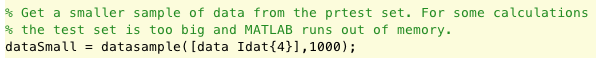
\includegraphics[scale=0.3]{smalldata.png}
        
        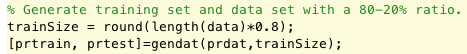
\includegraphics[scale=0.30]{training.png}
    \end{columns}
\end{frame}

%\subsection{Components}
%
%\begin{frame}{Analysing the data}{Components}
%    \begin{columns}
%    \column{0.6\textwidth}
%    \begin{itemize}
%        \item Plot components vs each other
%        \item \emph{All three plots shows the skin data (blue) grouped together vs the non-skin (red) more spread out. }
%    \end{itemize}
%    \column{0.4\textwidth}
%        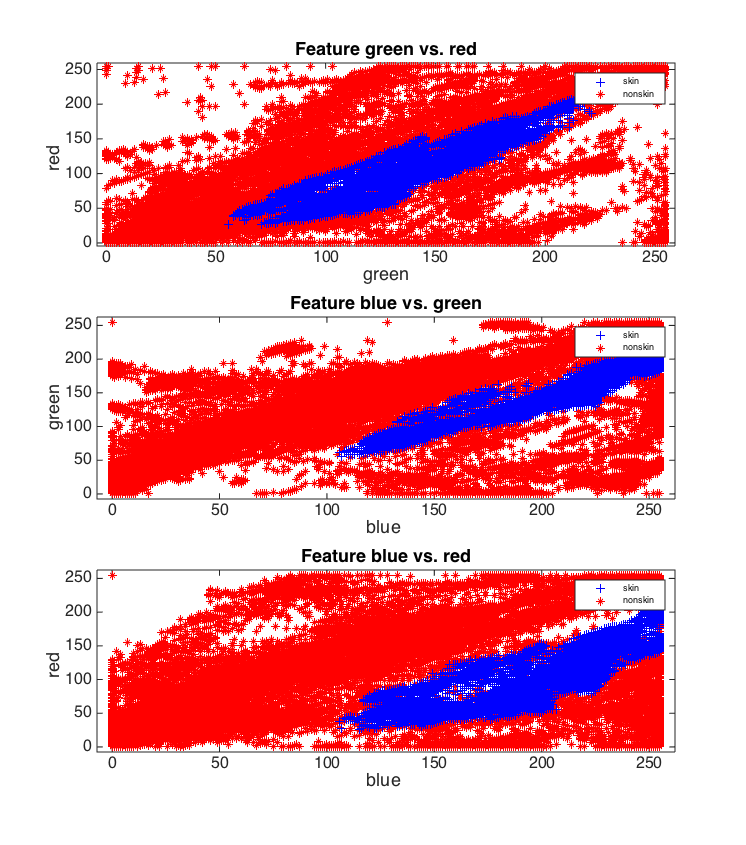
\includegraphics[scale=0.2]{components.png}
%    \end{columns}
%\end{frame}

\subsection{Correlation}

\begin{frame}{Analysing the data}{Correlation}
    \begin{columns}
    \column{0.6\textwidth}
    \begin{itemize}
        \item Correlation coefficients
        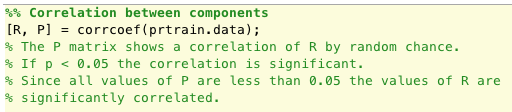
\includegraphics[scale=0.3]{correlation.png}
    \end{itemize}
    \column{0.4\textwidth}
        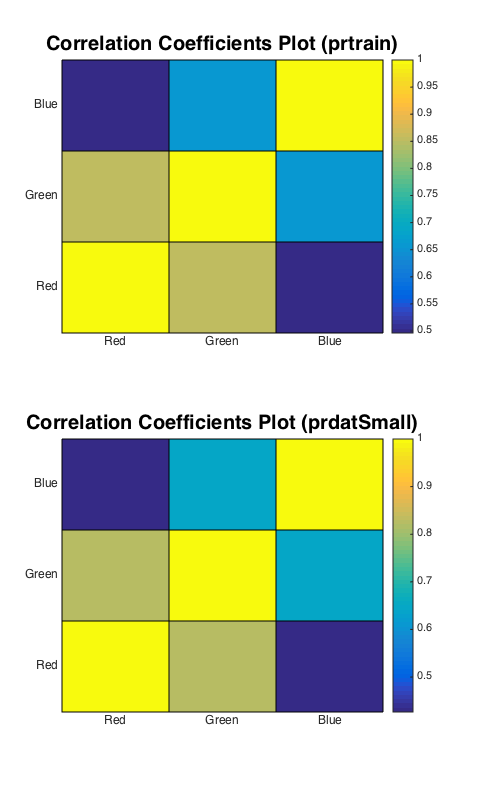
\includegraphics[scale=0.2]{CCplot.png}
    \end{columns}
\end{frame}

\begin{frame}{Analysing the data}{Principal Component Analysis}
    \begin{columns}
    \column{0.6\textwidth}
    \begin{itemize}
        \item PCA
        \item Cumulative Eigenvalues
        
        % This file was created by matlab2tikz.
% Minimal pgfplots version: 1.3
%
%The latest updates can be retrieved from
%  http://www.mathworks.com/matlabcentral/fileexchange/22022-matlab2tikz
%where you can also make suggestions and rate matlab2tikz.
%
\definecolor{mycolor1}{rgb}{0.00000,0.44700,0.74100}%
%
\tikzset{every picture/.append style={font=\tiny}}

\begin{tikzpicture}

\begin{axis}[%
width=1in,
height=0.8in,
at={(1.011111in,0.641667in)},
scale only axis,
xmin=1,
xmax=3,
xlabel={No of Principle Components},
ymin=0.75,
ymax=1,
ylabel shift=-20in, % new bit
ylabel={Percentage of Explained Variance},
title={Cumulative Eigenvalues (prtrain)}
]
\addplot [color=mycolor1,solid,forget plot]
  table[row sep=crcr]{%
1	0.770237860870193\\
2	0.965292133319316\\
3	1\\
};
\end{axis}
\end{tikzpicture}%
    \end{itemize}
    \column{0.4\textwidth}
        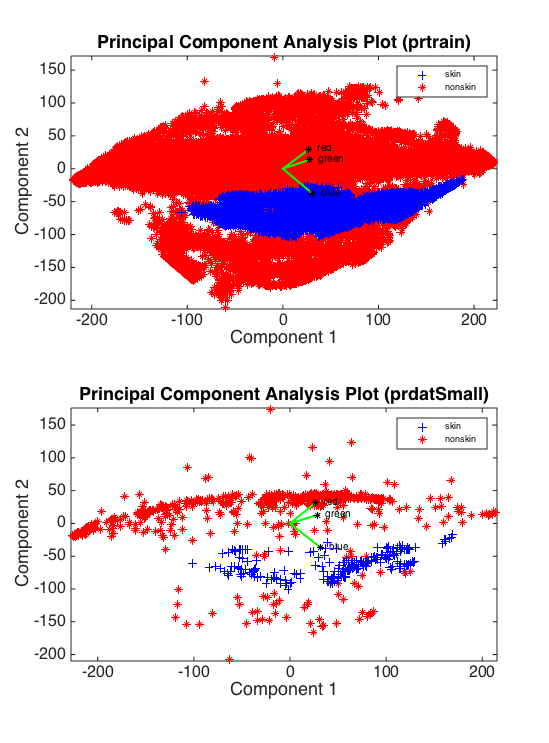
\includegraphics[scale=0.2]{PCAplot.png}
    \end{columns}
\end{frame}

\subsection{Feature Selection and Cluster Evaluation}

\begin{frame}{Analysing the data}{Feature Selection}
    \begin{columns}
    \column{0.7\textwidth}
    \begin{itemize}
        \item featselm(prtrain,ldc([]),'forward',2);
        \item \emph{Feature 1 (red) and 3 (blue) are selected.}
        \item featselm(prtrain,dtc([]),'forward',2);
        \item \emph{Feature 2 (green) and 3 (blue) are selected.}
    \end{itemize}
    \column{0.3\textwidth}
        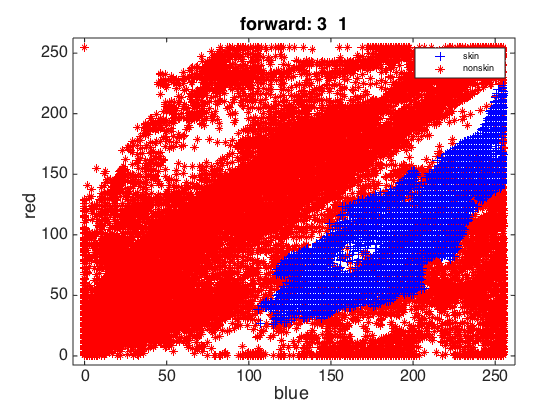
\includegraphics[scale=0.2]{featureselection.png}
    \end{columns}
\end{frame}

%\begin{frame}{Analysing the data}{Cluster Evaluation}
%    \begin{columns}
%   \column{0.5\textwidth}
%    \begin{itemize}
%        \item evalclusters(prdatSmall.data,
%        'kmeans','gap','KList',[1:15])
%        \item \emph{Long computation time}
%        \item \emph{Done on reduced dataset}
%    \end{itemize}
%    \column{0.5\textwidth}
%        % This file was created by matlab2tikz.
% Minimal pgfplots version: 1.3
%
%The latest updates can be retrieved from
%  http://www.mathworks.com/matlabcentral/fileexchange/22022-matlab2tikz
%where you can also make suggestions and rate matlab2tikz.
%
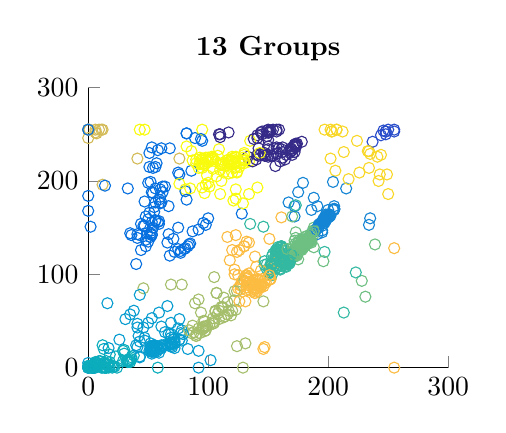
\begin{tikzpicture}

\begin{axis}[%
width=1.8in,
height=1.4in,
at={(1.011111in,0.641667in)},
scale only axis,
colormap={mymap}{[1pt] rgb(0pt)=(0.2081,0.1663,0.5292); rgb(1pt)=(0.211624,0.189781,0.577676); rgb(2pt)=(0.212252,0.213771,0.626971); rgb(3pt)=(0.2081,0.2386,0.677086); rgb(4pt)=(0.195905,0.264457,0.7279); rgb(5pt)=(0.170729,0.291938,0.779248); rgb(6pt)=(0.125271,0.324243,0.830271); rgb(7pt)=(0.0591333,0.359833,0.868333); rgb(8pt)=(0.0116952,0.38751,0.881957); rgb(9pt)=(0.00595714,0.408614,0.882843); rgb(10pt)=(0.0165143,0.4266,0.878633); rgb(11pt)=(0.0328524,0.443043,0.871957); rgb(12pt)=(0.0498143,0.458571,0.864057); rgb(13pt)=(0.0629333,0.47369,0.855438); rgb(14pt)=(0.0722667,0.488667,0.8467); rgb(15pt)=(0.0779429,0.503986,0.838371); rgb(16pt)=(0.0793476,0.520024,0.831181); rgb(17pt)=(0.0749429,0.537543,0.826271); rgb(18pt)=(0.0640571,0.556986,0.823957); rgb(19pt)=(0.0487714,0.577224,0.822829); rgb(20pt)=(0.0343429,0.596581,0.819852); rgb(21pt)=(0.0265,0.6137,0.8135); rgb(22pt)=(0.0238905,0.628662,0.803762); rgb(23pt)=(0.0230905,0.641786,0.791267); rgb(24pt)=(0.0227714,0.653486,0.776757); rgb(25pt)=(0.0266619,0.664195,0.760719); rgb(26pt)=(0.0383714,0.674271,0.743552); rgb(27pt)=(0.0589714,0.683757,0.725386); rgb(28pt)=(0.0843,0.692833,0.706167); rgb(29pt)=(0.113295,0.7015,0.685857); rgb(30pt)=(0.145271,0.709757,0.664629); rgb(31pt)=(0.180133,0.717657,0.642433); rgb(32pt)=(0.217829,0.725043,0.619262); rgb(33pt)=(0.258643,0.731714,0.595429); rgb(34pt)=(0.302171,0.737605,0.571186); rgb(35pt)=(0.348167,0.742433,0.547267); rgb(36pt)=(0.395257,0.7459,0.524443); rgb(37pt)=(0.44201,0.748081,0.503314); rgb(38pt)=(0.487124,0.749062,0.483976); rgb(39pt)=(0.530029,0.749114,0.466114); rgb(40pt)=(0.570857,0.748519,0.44939); rgb(41pt)=(0.609852,0.747314,0.433686); rgb(42pt)=(0.6473,0.7456,0.4188); rgb(43pt)=(0.683419,0.743476,0.404433); rgb(44pt)=(0.71841,0.741133,0.390476); rgb(45pt)=(0.752486,0.7384,0.376814); rgb(46pt)=(0.785843,0.735567,0.363271); rgb(47pt)=(0.818505,0.732733,0.34979); rgb(48pt)=(0.850657,0.7299,0.336029); rgb(49pt)=(0.882433,0.727433,0.3217); rgb(50pt)=(0.913933,0.725786,0.306276); rgb(51pt)=(0.944957,0.726114,0.288643); rgb(52pt)=(0.973895,0.731395,0.266648); rgb(53pt)=(0.993771,0.745457,0.240348); rgb(54pt)=(0.999043,0.765314,0.216414); rgb(55pt)=(0.995533,0.786057,0.196652); rgb(56pt)=(0.988,0.8066,0.179367); rgb(57pt)=(0.978857,0.827143,0.163314); rgb(58pt)=(0.9697,0.848138,0.147452); rgb(59pt)=(0.962586,0.870514,0.1309); rgb(60pt)=(0.958871,0.8949,0.113243); rgb(61pt)=(0.959824,0.921833,0.0948381); rgb(62pt)=(0.9661,0.951443,0.0755333); rgb(63pt)=(0.9763,0.9831,0.0538)},
xmin=0,
xmax=300,
ymin=0,
ymax=300,
title style={font=\bfseries},
title={13 Groups},
axis x line*=bottom,
axis y line*=left
]
\addplot[scatter,only marks,scatter src=explicit,scatter/use mapped color={mark=o,mark options={},draw=mapped color}] plot table[row sep=crcr,meta index=2]{%
92	148	3\\
181	138	8\\
67	24	5\\
54	21	5\\
40	111	3\\
172	162	4\\
199	162	4\\
170	120	7\\
167	115	7\\
178	130	8\\
127	89	11\\
110	218	13\\
195	145	4\\
151	105	7\\
178	133	8\\
12	24	6\\
160	221	1\\
163	117	7\\
98	40	9\\
175	125	8\\
234	214	12\\
1	255	10\\
199	162	4\\
172	121	8\\
181	135	8\\
178	131	8\\
198	158	4\\
33	8	6\\
98	44	9\\
20	0	6\\
174	240	1\\
164	114	7\\
132	135	11\\
161	161	11\\
197	158	4\\
15	0	6\\
10	4	6\\
78	40	5\\
178	242	1\\
95	243	3\\
185	135	8\\
181	136	8\\
175	124	8\\
134	134	11\\
57	219	3\\
178	128	8\\
97	187	13\\
104	53	9\\
172	136	8\\
54	18	5\\
125	99	11\\
173	237	1\\
111	217	13\\
157	120	7\\
187	146	4\\
29	7	6\\
78	89	9\\
107	80	9\\
157	255	1\\
168	112	7\\
104	224	13\\
162	231	1\\
150	228	1\\
161	130	7\\
132	96	11\\
165	118	7\\
129	223	13\\
166	112	7\\
198	164	4\\
90	34	9\\
191	173	4\\
18	6	6\\
166	117	7\\
33	7	6\\
89	69	9\\
152	95	11\\
178	130	8\\
144	88	11\\
156	106	7\\
78	29	5\\
133	90	11\\
140	88	11\\
178	132	8\\
47	178	3\\
132	83	11\\
48	162	3\\
6	255	10\\
172	127	8\\
234	153	4\\
163	113	7\\
177	129	8\\
43	11	5\\
178	128	8\\
160	129	7\\
153	99	7\\
167	113	7\\
138	82	11\\
42	34	5\\
185	142	8\\
178	128	8\\
54	23	5\\
178	133	8\\
134	221	13\\
52	20	5\\
165	115	7\\
164	114	7\\
199	163	4\\
207	255	12\\
215	192	4\\
173	122	8\\
119	222	13\\
72	28	5\\
55	24	5\\
172	122	8\\
136	90	11\\
180	134	8\\
235	160	4\\
129	222	13\\
170	118	7\\
177	134	8\\
203	253	12\\
51	166	3\\
2	151	3\\
175	125	8\\
144	252	1\\
116	217	13\\
123	62	9\\
175	125	8\\
160	106	7\\
139	119	11\\
175	125	8\\
121	179	13\\
139	90	11\\
179	132	8\\
178	128	8\\
161	129	7\\
157	126	7\\
133	226	1\\
205	170	4\\
171	130	8\\
61	21	5\\
7	5	6\\
181	134	8\\
143	229	1\\
127	88	11\\
175	127	8\\
175	127	8\\
33	192	3\\
151	101	7\\
142	93	11\\
170	233	1\\
201	164	4\\
178	131	8\\
205	169	4\\
152	110	7\\
72	124	3\\
161	130	7\\
17	2	6\\
163	128	7\\
153	227	1\\
4	0	6\\
23	12	6\\
76	52	5\\
255	0	11\\
156	216	1\\
188	150	8\\
197	124	7\\
180	130	8\\
0	0	6\\
178	131	8\\
158	126	7\\
194	155	4\\
111	65	9\\
205	173	4\\
93	218	13\\
195	147	4\\
176	126	8\\
173	133	8\\
165	108	7\\
161	130	7\\
55	17	5\\
151	94	11\\
68	235	3\\
92	73	9\\
109	52	9\\
95	43	9\\
105	97	9\\
165	117	7\\
107	205	13\\
170	127	8\\
35	57	5\\
160	105	7\\
169	234	1\\
110	250	1\\
164	114	7\\
123	181	13\\
164	110	7\\
53	19	5\\
8	5	5\\
172	125	8\\
170	162	8\\
173	240	1\\
71	138	3\\
195	156	4\\
106	60	9\\
199	160	4\\
201	162	4\\
175	128	8\\
217	202	12\\
154	105	7\\
150	252	1\\
201	162	4\\
174	121	8\\
176	131	8\\
36	142	3\\
60	183	3\\
6	0	6\\
109	250	1\\
182	135	8\\
81	191	13\\
195	156	4\\
55	23	5\\
18	14	6\\
158	118	7\\
198	162	4\\
41	143	3\\
124	82	9\\
104	213	13\\
41	224	10\\
75	150	3\\
135	83	11\\
161	123	8\\
201	162	4\\
178	131	8\\
175	125	8\\
188	129	8\\
133	97	11\\
188	143	8\\
141	249	1\\
98	223	13\\
160	121	7\\
112	64	9\\
140	108	11\\
158	129	7\\
180	132	8\\
183	135	8\\
146	229	1\\
175	116	8\\
138	89	11\\
110	186	13\\
36	11	6\\
180	133	8\\
38	13	6\\
130	228	13\\
14	0	6\\
0	5	5\\
201	164	4\\
178	128	8\\
83	130	3\\
66	134	3\\
56	158	3\\
111	200	13\\
123	215	13\\
188	147	8\\
179	129	8\\
69	25	5\\
24	0	6\\
163	112	7\\
248	253	2\\
176	137	8\\
183	138	8\\
137	91	11\\
46	152	3\\
10	7	6\\
14	0	6\\
141	95	11\\
122	218	13\\
175	129	8\\
131	222	13\\
44	126	3\\
151	253	1\\
177	134	8\\
179	198	4\\
128	88	11\\
178	131	8\\
181	131	8\\
100	225	13\\
158	230	1\\
186	169	4\\
109	234	13\\
41	43	5\\
103	226	13\\
53	142	3\\
41	22	5\\
196	156	4\\
122	100	11\\
159	123	7\\
200	163	4\\
175	188	4\\
152	103	7\\
81	128	3\\
55	22	5\\
150	244	1\\
170	118	7\\
157	126	7\\
48	130	3\\
173	145	8\\
195	152	4\\
226	209	12\\
234	232	12\\
175	125	8\\
235	229	12\\
196	114	8\\
132	86	11\\
48	137	3\\
13	5	6\\
104	225	13\\
80	127	3\\
116	57	9\\
146	87	11\\
173	123	8\\
135	243	13\\
53	156	3\\
90	223	13\\
202	163	4\\
136	90	11\\
118	115	11\\
178	131	8\\
140	90	11\\
181	133	8\\
180	130	8\\
43	28	5\\
77	37	5\\
9	255	10\\
30	19	6\\
244	228	12\\
88	38	9\\
179	129	8\\
59	157	3\\
152	227	1\\
53	22	5\\
201	162	4\\
141	246	1\\
66	25	5\\
54	22	5\\
69	32	5\\
197	155	4\\
141	228	1\\
156	119	7\\
43	255	13\\
75	42	5\\
160	106	7\\
172	122	8\\
4	0	6\\
53	53	5\\
53	15	5\\
173	239	1\\
3	0	6\\
96	218	13\\
179	131	8\\
87	45	9\\
132	99	11\\
202	255	12\\
161	109	7\\
57	21	5\\
157	115	7\\
61	235	3\\
182	135	8\\
162	225	1\\
86	37	9\\
141	85	11\\
62	23	5\\
129	0	9\\
157	229	1\\
199	160	4\\
170	228	1\\
184	134	8\\
87	146	3\\
55	22	5\\
179	132	8\\
148	227	1\\
142	235	1\\
177	127	8\\
172	119	7\\
130	219	13\\
110	212	13\\
99	206	13\\
158	122	7\\
59	16	5\\
85	133	3\\
0	2	6\\
180	130	8\\
201	162	4\\
241	226	12\\
150	252	1\\
145	250	1\\
255	255	2\\
57	17	5\\
172	122	8\\
130	93	9\\
67	173	3\\
178	132	8\\
3	0	6\\
184	136	8\\
107	80	9\\
178	131	8\\
122	72	9\\
249	207	12\\
90	36	9\\
54	187	3\\
198	161	4\\
35	8	6\\
100	160	3\\
57	23	5\\
123	191	13\\
172	173	4\\
192	153	4\\
178	131	8\\
82	180	3\\
26	30	5\\
149	105	7\\
63	24	5\\
6	3	6\\
196	157	4\\
127	84	11\\
178	131	8\\
43	12	5\\
168	114	7\\
104	47	9\\
198	159	4\\
84	132	3\\
171	125	8\\
46	43	5\\
0	168	3\\
61	21	5\\
139	80	11\\
61	177	3\\
201	164	4\\
140	223	1\\
95	41	9\\
175	134	8\\
108	58	9\\
151	252	1\\
170	124	8\\
150	252	1\\
242	200	12\\
172	124	8\\
163	112	7\\
53	143	3\\
81	189	3\\
152	95	11\\
196	159	4\\
4	0	6\\
145	89	11\\
205	170	4\\
197	160	4\\
183	136	8\\
140	88	11\\
149	248	1\\
13	20	6\\
164	113	7\\
181	134	8\\
53	20	5\\
56	215	3\\
200	163	4\\
147	93	11\\
2	1	6\\
1	1	6\\
144	86	11\\
151	106	11\\
98	153	3\\
136	90	11\\
0	0	5\\
197	160	4\\
165	115	7\\
237	242	2\\
57	23	5\\
193	154	4\\
54	21	5\\
0	255	3\\
131	98	11\\
197	160	4\\
134	92	11\\
70	25	5\\
167	177	4\\
146	71	9\\
181	135	8\\
189	146	4\\
4	2	6\\
162	120	7\\
9	2	6\\
182	135	8\\
116	222	13\\
198	161	4\\
166	118	7\\
4	0	6\\
156	125	7\\
122	82	9\\
128	165	3\\
113	220	13\\
188	147	8\\
182	135	8\\
174	121	8\\
21	1	6\\
54	150	3\\
163	115	7\\
191	143	4\\
50	48	5\\
122	214	13\\
174	120	8\\
120	209	13\\
132	86	11\\
141	193	13\\
101	46	9\\
31	52	5\\
51	230	3\\
97	219	13\\
75	209	3\\
137	221	1\\
175	125	8\\
147	22	11\\
22	1	6\\
182	132	8\\
199	162	4\\
178	128	8\\
6	252	10\\
89	246	3\\
155	235	1\\
149	254	1\\
82	251	3\\
184	138	8\\
172	239	1\\
69	89	9\\
79	36	5\\
185	137	8\\
165	228	1\\
138	84	11\\
68	25	5\\
172	124	8\\
53	19	5\\
55	22	5\\
53	17	5\\
185	139	8\\
198	162	4\\
86	211	3\\
181	140	8\\
67	143	3\\
98	196	13\\
190	148	4\\
161	112	7\\
83	20	5\\
53	188	3\\
177	129	8\\
47	32	5\\
246	254	2\\
123	142	11\\
201	162	4\\
85	192	13\\
97	217	13\\
82	237	13\\
178	128	8\\
205	170	4\\
52	21	5\\
197	160	4\\
174	129	8\\
51	215	3\\
9	7	6\\
145	253	1\\
147	114	7\\
76	207	3\\
127	219	13\\
228	93	8\\
178	126	8\\
197	157	4\\
99	221	13\\
198	158	4\\
162	110	7\\
165	115	7\\
60	191	3\\
35	144	3\\
171	237	1\\
59	180	3\\
192	151	4\\
93	225	13\\
178	132	8\\
135	154	7\\
117	220	13\\
122	105	11\\
5	4	6\\
47	255	13\\
177	127	8\\
176	130	8\\
139	80	11\\
173	236	1\\
125	85	11\\
15	0	6\\
164	113	7\\
151	99	11\\
206	211	12\\
213	59	7\\
186	134	8\\
203	253	12\\
118	221	13\\
146	20	11\\
55	24	5\\
170	119	7\\
148	91	11\\
106	221	13\\
178	128	8\\
95	193	13\\
192	150	4\\
69	48	5\\
94	59	9\\
196	159	4\\
164	113	7\\
158	114	7\\
55	172	3\\
181	134	8\\
18	1	6\\
84	40	9\\
181	133	8\\
141	82	11\\
179	129	8\\
55	22	5\\
82	251	3\\
0	1	6\\
0	246	10\\
204	169	4\\
114	55	9\\
197	158	4\\
96	155	3\\
95	218	13\\
182	135	8\\
154	108	7\\
6	2	6\\
198	161	4\\
168	118	7\\
178	131	8\\
116	70	9\\
52	140	3\\
151	105	7\\
97	39	9\\
180	132	8\\
56	157	3\\
188	182	4\\
53	17	5\\
166	112	7\\
172	120	8\\
132	99	11\\
56	192	3\\
213	231	12\\
163	112	7\\
55	24	5\\
36	9	6\\
120	222	13\\
5	0	5\\
163	115	7\\
132	92	11\\
119	56	9\\
223	102	7\\
53	236	3\\
175	127	8\\
201	162	4\\
59	154	3\\
17	0	6\\
96	42	9\\
158	113	11\\
117	252	1\\
130	222	13\\
62	188	3\\
46	85	9\\
142	227	1\\
61	24	5\\
171	123	8\\
180	132	8\\
103	223	13\\
86	232	13\\
199	163	4\\
67	36	5\\
199	162	4\\
198	158	4\\
160	129	7\\
126	215	13\\
130	130	11\\
134	101	11\\
117	208	13\\
186	136	8\\
169	123	7\\
163	114	7\\
12	255	10\\
173	125	8\\
177	129	8\\
47	152	3\\
6	5	6\\
162	112	7\\
178	128	8\\
162	236	1\\
157	253	1\\
176	126	8\\
175	134	8\\
158	127	7\\
182	141	8\\
0	0	5\\
98	225	13\\
239	132	8\\
58	156	3\\
166	116	7\\
154	255	1\\
150	255	1\\
143	94	11\\
180	135	8\\
126	71	11\\
170	124	8\\
167	120	7\\
150	226	1\\
12	0	6\\
159	235	1\\
1	0	6\\
176	126	8\\
129	176	13\\
165	114	7\\
124	210	13\\
141	95	11\\
193	154	4\\
90	219	13\\
243	207	12\\
150	237	1\\
35	6	6\\
179	129	8\\
69	26	5\\
255	253	2\\
124	209	13\\
95	223	13\\
184	135	8\\
157	236	1\\
122	221	13\\
167	111	7\\
76	30	5\\
0	255	10\\
58	233	3\\
154	122	7\\
185	137	8\\
34	7	6\\
71	30	5\\
70	27	5\\
139	93	11\\
150	234	1\\
51	18	5\\
171	121	7\\
15	7	6\\
58	0	6\\
69	36	5\\
205	170	4\\
120	224	13\\
155	109	7\\
199	162	4\\
55	18	5\\
172	121	8\\
168	114	7\\
139	86	11\\
72	31	5\\
52	199	3\\
169	232	1\\
179	128	8\\
174	124	8\\
126	126	11\\
76	224	10\\
175	125	8\\
77	125	3\\
12	196	10\\
172	121	8\\
143	89	11\\
202	224	12\\
66	66	5\\
50	159	3\\
134	91	11\\
66	24	5\\
102	222	13\\
6	6	6\\
55	22	5\\
199	162	4\\
248	250	2\\
44	154	3\\
10	4	6\\
147	230	1\\
96	50	9\\
0	255	10\\
199	162	4\\
102	8	5\\
172	231	1\\
3	2	6\\
93	220	13\\
124	23	9\\
192	150	4\\
179	129	8\\
142	89	11\\
136	90	11\\
77	123	3\\
197	160	4\\
173	174	7\\
183	138	8\\
30	15	6\\
153	111	7\\
43	142	3\\
17	21	5\\
14	195	3\\
177	129	8\\
163	113	7\\
7	251	10\\
50	135	3\\
53	147	3\\
161	234	1\\
92	42	9\\
76	30	5\\
181	134	8\\
100	198	13\\
174	124	8\\
151	138	11\\
16	4	6\\
11	255	10\\
112	65	9\\
197	158	4\\
2	1	6\\
153	119	7\\
5	0	6\\
196	157	4\\
159	255	1\\
123	226	13\\
130	222	13\\
0	184	3\\
158	108	7\\
186	144	8\\
95	255	13\\
16	69	5\\
50	198	3\\
99	45	9\\
184	136	8\\
146	151	7\\
56	177	3\\
52	26	5\\
114	216	13\\
131	26	9\\
54	214	3\\
90	34	9\\
175	125	8\\
152	111	7\\
200	163	4\\
33	6	6\\
244	249	2\\
168	230	1\\
72	21	5\\
69	23	5\\
29	18	6\\
113	209	13\\
248	253	2\\
130	130	11\\
103	224	13\\
124	124	11\\
168	114	7\\
231	76	8\\
49	144	3\\
180	135	8\\
95	224	13\\
0	0	6\\
161	126	7\\
160	115	7\\
173	122	8\\
144	88	11\\
162	115	7\\
55	167	3\\
138	245	1\\
41	47	5\\
182	135	8\\
181	131	8\\
52	18	5\\
52	18	5\\
161	109	7\\
100	220	13\\
62	194	3\\
197	255	12\\
14	0	6\\
157	126	7\\
97	50	9\\
152	254	1\\
117	223	13\\
20	2	6\\
60	21	5\\
212	253	12\\
164	112	7\\
178	130	8\\
250	186	12\\
2	2	6\\
131	71	11\\
96	44	9\\
52	144	3\\
153	110	7\\
153	111	7\\
106	61	9\\
16	3	6\\
179	131	8\\
134	88	11\\
41	139	3\\
64	194	3\\
40	24	5\\
173	238	1\\
123	225	13\\
169	235	1\\
117	61	9\\
178	137	8\\
93	37	9\\
139	84	11\\
198	158	4\\
129	225	13\\
122	219	13\\
185	142	8\\
120	126	11\\
11	0	6\\
120	220	13\\
183	138	8\\
109	61	9\\
178	137	8\\
169	121	7\\
47	29	5\\
52	23	5\\
139	90	11\\
137	91	11\\
224	243	12\\
165	109	7\\
151	102	7\\
255	128	11\\
68	120	3\\
159	123	7\\
61	44	5\\
174	124	8\\
112	218	13\\
143	230	13\\
172	121	8\\
147	110	7\\
182	134	8\\
129	94	11\\
64	38	5\\
178	127	8\\
181	138	8\\
130	230	13\\
32	7	6\\
113	54	9\\
72	26	5\\
134	186	13\\
92	0	5\\
58	19	5\\
199	162	4\\
166	127	8\\
101	194	13\\
172	121	8\\
164	223	1\\
92	18	5\\
94	245	3\\
188	146	8\\
156	120	7\\
144	104	11\\
147	227	1\\
59	59	5\\
250	255	2\\
113	75	9\\
110	247	1\\
144	87	11\\
120	226	13\\
173	139	8\\
95	214	13\\
0	255	3\\
207	255	12\\
200	169	4\\
167	115	7\\
197	157	4\\
98	44	9\\
180	135	8\\
132	95	11\\
233	232	12\\
104	49	9\\
149	111	7\\
43	78	5\\
204	199	4\\
196	157	4\\
152	254	1\\
120	61	9\\
70	22	5\\
116	140	11\\
151	99	11\\
145	95	11\\
76	197	13\\
60	176	3\\
92	214	13\\
75	127	3\\
38	61	5\\
167	113	7\\
2	0	6\\
105	48	9\\
87	222	13\\
201	162	4\\
108	227	13\\
};
\end{axis}
\end{tikzpicture}%
%    \end{columns}
%\end{frame}

\section{Classification}
\subsection{Parametric and Non-Parametric}
\begin{frame}{Classification}{Parametric and Non-Parametric}
    \begin{columns}
    \column{0.5\textwidth}
    \begin{itemize}
        \item Parametric: \emph{ldc, qdc, nmc, fisherc}
        \item Non-Parametric: \emph{dtc, parzenc, knnc, svc}
        \item Long computation time $\rightarrow$ smaller dataset.
    \end{itemize}
    \column{0.5\textwidth}
        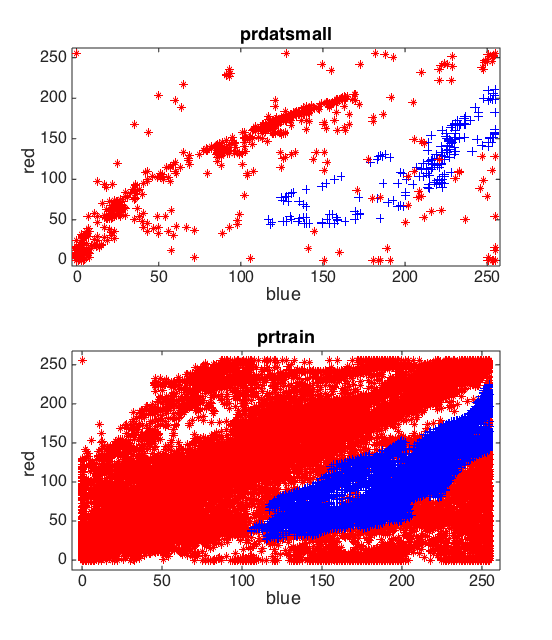
\includegraphics[scale=0.3]{prdat.png}
    \end{columns}
\end{frame}

\begin{frame}{Classification}{9 Classification methods}
    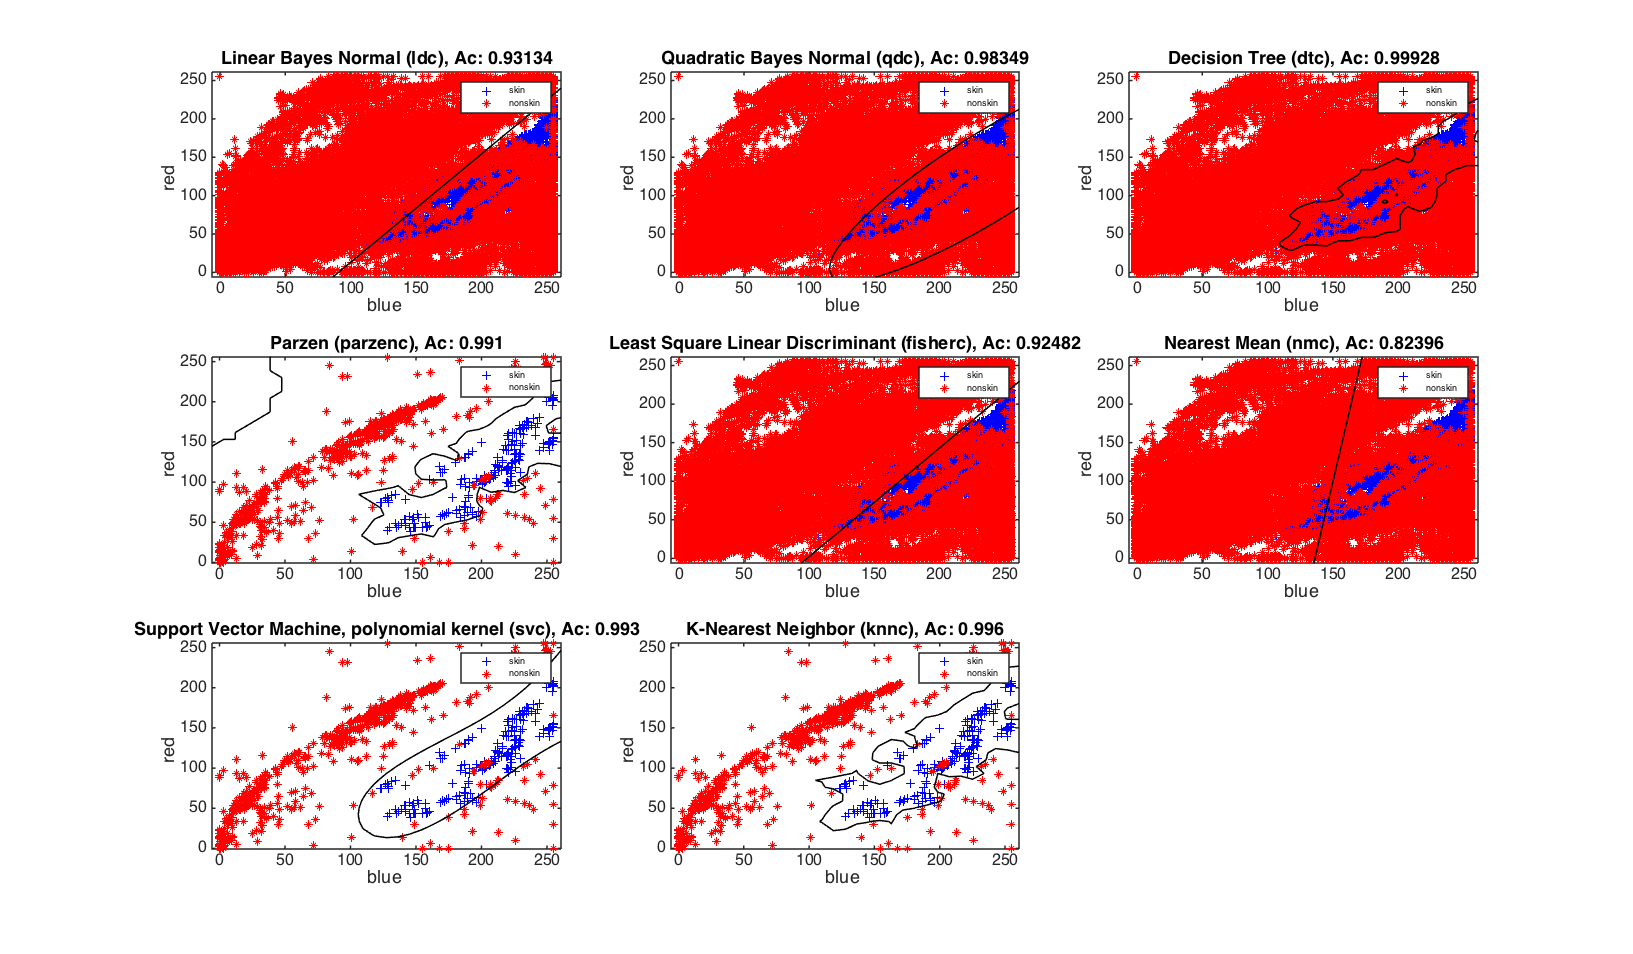
\includegraphics[scale=0.2]{fullnew8.png}
\end{frame}


\definecolor{Green}{RGB}{46, 204, 113}
\definecolor{Red}{RGB}{231, 76, 60}
\definecolor{Gray}{RGB}{149, 165, 166}
\definecolor{Cloud}{RGB}{236, 240, 241}

\newcolumntype{g}{>{\columncolor{Green}}c}
\newcolumntype{r}{>{\columncolor{Red}}c}
\newcolumntype{y}{>{\columncolor{Gray}}c}
\newcolumntype{l}{>{\columncolor{Cloud}}c}

\begin{frame}{Classification}{Accuracy / Crossvalidation}
    \begin{table}
    \resizebox{\columnwidth}{!}{%
        \begin{tabular}{c|c|c|g|c|c|r|l|l}
        & ldc & qdc & dtc & parzenc & fisherc  & nmc & svc & knnc \\ \hline
        ac & 0.9313 & 0.9835 & 0.9993 & 0.9910 & 0.9248 & 0.8240 & 0.9930 & 0.9960 \\ \hline
        time &  6.11s & 7.45s & 53.12s & 20.76s & 9.91s & 15.27s & 20.37s & 26.33s \\ \hline 
        & & & best &  & & worst & second & third
        \end{tabular}
    }
    \end{table}
    \begin{center}
    %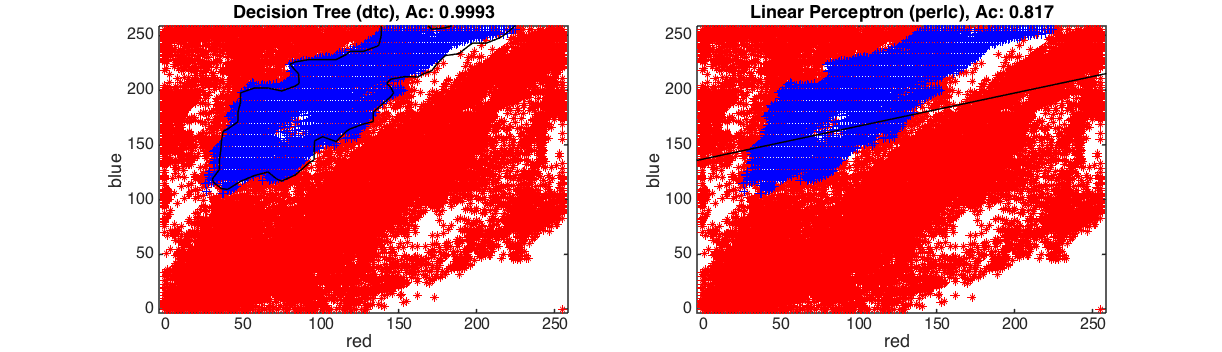
\includegraphics[scale=0.25]{bestworst.png}
    \begin{columns}
    \column{0.5\textwidth}
        \centering 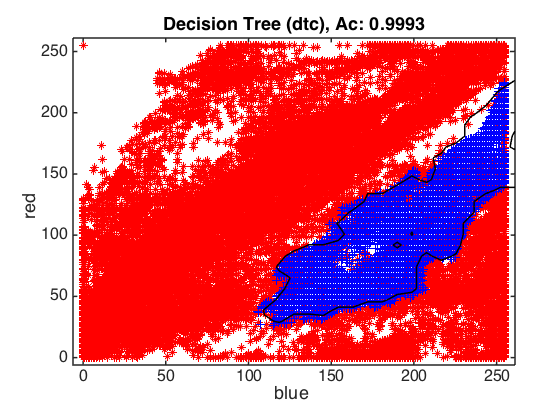
\includegraphics[scale=0.25]{dtc.png}
    \column{0.5\textwidth}
        \centering 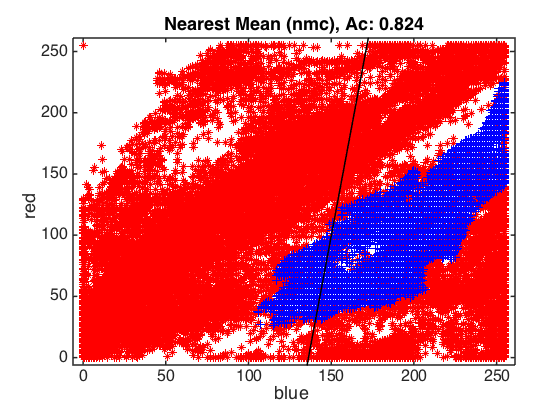
\includegraphics[scale=0.25]{nmc.png}
    \end{columns}
    \end{center}
\end{frame}

\end{document}


